\documentclass[10pt,twocolumn,letterpaper]{article}
\usepackage[T1]{fontenc}
\usepackage[utf8]{inputenc}
\usepackage{mathptmx}
\usepackage[letterpaper,top=0.8in,bottom=0.8in,left=0.7in,right=0.7in,columnsep=0.28in,headsep=0.2in]{geometry}
\usepackage{graphicx}
\usepackage{booktabs,longtable,tabularx,array,multirow}
\usepackage[font=small,labelfont=bf,labelsep=period,justification=justified,singlelinecheck=false]{caption}
\usepackage{fancyhdr}
\usepackage[dvipsnames]{xcolor}
\usepackage[numbers,sort&compress,square,comma]{natbib}
\usepackage{titlesec}
\usepackage{enumitem}
\usepackage{microtype}
\usepackage{lastpage}
\usepackage{xurl}
\usepackage[colorlinks=true,linkcolor=MidnightBlue,citecolor=MidnightBlue,urlcolor=MidnightBlue]{hyperref}
\usepackage{doi}
\renewcommand{\doitext}{doi:}

% ---------- headings (ODP-style: centered, bold, uppercase) ----------
\titleformat{\section}{\normalfont\normalsize\bfseries\centering}{\thesection.}{0.5em}{\MakeUppercase}
\titlespacing*{\section}{0pt}{1.2ex plus .5ex}{0.8ex}
\titleformat{\subsection}{\normalfont\normalsize\bfseries}{\thesubsection}{0.5em}{}
\titlespacing*{\subsection}{0pt}{1.0ex plus .4ex}{0.4ex}
\setlength{\parindent}{1.2em}

% ---------- running header ----------
\pagestyle{fancy}
\fancyhf{}
\fancyhead[L]{\footnotesize B.\,K. DANSO, J.\,O. DANKWA, AND A.\,A. AIDOO}
\fancyhead[R]{\footnotesize FERTILE OR BARREN: AN OPEN Ni-Cu-PGE FERTILITY BENCHMARK \quad \thepage}
\renewcommand{\headrulewidth}{0.4pt}
\fancypagestyle{first}{\fancyhf{}\renewcommand{\headrulewidth}{0pt}
  \fancyhead[L]{\footnotesize Preprint (not peer reviewed). Version 1, October 2026.}
  \fancyfoot[C]{\footnotesize \thepage\ of \pageref{LastPage}}}

\captionsetup[figure]{name=Figure}
\setlength{\abovecaptionskip}{4pt}
\renewcommand{\topfraction}{0.92}\renewcommand{\dbltopfraction}{0.92}\renewcommand{\textfraction}{0.08}
\renewcommand{\floatpagefraction}{0.8}\renewcommand{\dblfloatpagefraction}{0.8}
\setcounter{dbltopnumber}{3}\setcounter{topnumber}{3}
\setlength{\textfloatsep}{10pt plus 2pt minus 2pt}
\setlength{\dbltextfloatsep}{10pt plus 2pt minus 2pt}
\renewcommand{\bibfont}{\small}
\setlength{\bibsep}{1.5pt}
\newcommand{\orcid}[1]{\href{https://orcid.org/#1}{#1}}

\hypersetup{pdftitle={Fertile or Barren: an open benchmark for testing geochemical fertility indices on mineralized and barren mafic-ultramafic intrusions},
pdfauthor={Bezali Kwame Danso, Josephine Opare Dankwa, Adwoa Aduaba Aidoo}}

\makeatletter\newcommand\tabinput[1]{\@@input #1 }\makeatother
\begin{document}

% ---------------- cover page ----------------
\begin{titlepage}
\vspace*{0.9in}
\begin{center}\large
{\LARGE\bfseries Fertile or Barren: an open benchmark for testing geochemical fertility indices on mineralized and barren mafic-ultramafic intrusions\par}
\vspace{24pt}
{\fontsize{12.5}{16}\selectfont
{\bfseries Bezali Kwame Danso$^{*}$\par}
Independent Researcher, East Lansing, Michigan, USA\\
Email: \href{mailto:dansobez@msu.edu}{dansobez@msu.edu}\\
ORCID: \orcid{0009-0006-1201-4129}
\vspace{12pt}

{\bfseries Josephine Opare Dankwa\par}
Independent Researcher, Springfield, Missouri, USA\\
ORCID: \orcid{0009-0000-6105-1213}
\vspace{12pt}

{\bfseries Adwoa Aduaba Aidoo\par}
Independent Researcher, Mine Geologist, Benso, Ghana\\
ORCID: \orcid{0009-0000-4363-8651}\par}
\end{center}
\vspace{24pt}
\noindent{\large $^{*}$Corresponding author.}

\vspace{22pt}
\noindent\fbox{\parbox{\dimexpr\textwidth-2\fboxsep-2\fboxrule}{\large
This manuscript is a \textbf{preprint} and has \textbf{not been peer reviewed}. It has been submitted to EarthArXiv. It has not yet been submitted to a journal for peer review. Subsequent versions of this manuscript may have slightly different content.}}

\vspace{26pt}
\noindent{\large\textbf{Data and code.} Benchmark data, curated intrusion labels, scoring program and leaderboard (Fertile or Barren v0.1.0): \doi{10.5281/zenodo.23777406};\\ repository: \url{https://github.com/bkdanso/fertile-or-barren}.\par}
\end{titlepage}
\setcounter{page}{1}

\twocolumn[
\begin{center}
{\large\bfseries FERTILE OR BARREN: AN OPEN BENCHMARK FOR TESTING GEOCHEMICAL FERTILITY INDICES ON MINERALIZED AND BARREN MAFIC-ULTRAMAFIC INTRUSIONS\par}
\vspace{10pt}
{\normalsize Bezali Kwame Danso,$^{1,*}$ Josephine Opare Dankwa,$^{2}$ and Adwoa Aduaba Aidoo$^{3}$\par}
\vspace{12pt}
{\normalsize\bfseries ABSTRACT\par}
\end{center}
\vspace{-2pt}
\begin{list}{}{\leftmargin=0.55in\rightmargin=0.55in}\item\relax\small
Magmatic Ni-Cu-PGE sulfide deposits form through a sequence of processes (e.g., magma generation, transport, crustal interaction, sulfur saturation, and sulfide accumulation). These processes can modify whole-rock compositions in different ways, making it challenging to evaluate the geochemical fertility of mafic-ultramafic magmatic intrusions. Several whole-rock fertility indices have been proposed to identify intrusions capable of hosting magmatic sulfide mineralization, yet their performance is rarely assessed using a common dataset and consistent sampling criteria. We present \textit{Fertile or Barren}, an open benchmark assembled from GEOROC 2.0 compilations and U.S. Geological Survey deposit databases to evaluate published geochemical fertility indices for magmatic Ni-Cu-PGE systems. We identified 31,886 mafic-ultramafic plutonic samples, including 13,025 samples from 514 named intrusions represented by at least five analyses from 521,961 analyses. Intrusions were classified as fertile, weakly mineralized or barren and individual samples were assigned to petrologic categories including cumulate, chilled margin, fine-grained dike/sill, altered, and unresolved. We developed a public scoring workflow that evaluates each index using intrusion-weighted receiver operating characteristic (ROC) area-under-the-curve (AUC) statistics with bootstrap confidence intervals. Three indices (Ni/Cu, Ni depletion relative to MgO, and Cu/Zr) performed significantly below random expectation (AUC $<$ 0.5), ranking barren intrusions above fertile ones. For depletion-based indices, this result is consistent with the predominance of sulfide-bearing cumulates in the fertile dataset, which comprise 65\% of all fertile samples, rather than the sulfide-poor magma compositions these indices were originally designed to evaluate. This work provides a reproducible framework for evaluating existing geochemical fertility indices and identifying the geological and sampling conditions under which their application is most defensible by combining intrusion-level mineralization labels with sample-level petrologic classifications.

\vspace{4pt}
\textbf{Keywords:} critical minerals; magmatic sulfide deposits; Ni-Cu-PGE; geochemical fertility; GEOROC; exploration geochemistry; magma fertility; benchmark dataset.
\end{list}
\vspace{14pt}
]

\thispagestyle{first}
{\renewcommand{\thefootnote}{}\footnotetext{\hspace{-1.4em}\footnotesize
$^{1}$Independent Researcher, East Lansing, Michigan, USA. ORCID \orcid{0009-0006-1201-4129}.\\
$^{2}$Independent Researcher, Springfield, Missouri, USA. ORCID \orcid{0009-0000-6105-1213}.\\
$^{3}$Independent Researcher, Mine Geologist, Benso, Ghana. ORCID \orcid{0009-0000-4363-8651}.\\
$^{*}$Corresponding author: Bezali Kwame Danso, \href{mailto:dansobez@msu.edu}{dansobez@msu.edu}.\\
Data and code: \doi{10.5281/zenodo.23777406}; \url{https://github.com/bkdanso/fertile-or-barren}.}}

% =====================================================================
\section{Introduction}

Magmatic nickel-copper-platinum-group element (Ni-Cu-PGE) sulfide deposits constitute the world's principal source of nickel and platinum-group elements and an important source of cobalt \cite{mudd2014,naldrett2004}, commodities that are increasingly important for energy, transportation, and defense technologies. These economic metals get enriched when mantle-derived mafic to ultramafic magmas become saturated in sulfur, segregate an immiscible sulfide liquid, and subsequently concentrate that liquid into mineralized accumulations. Because Ni, Cu, and the PGE partition strongly into sulfide relative to silicate melt, the formation, transport, and accumulation of sulfide liquid can produce large variations in metal tenor among otherwise related magmas and intrusive bodies. Therefore, Ni-Cu-PGE deposit formation depends on a sequence of interconnected processes including magma generation, magma transport, crustal interaction, sulfide saturation, and sulfide accumulation, rather than on any single characteristic of a parental magma \cite{barneslightfoot2005,naldrett2010}.

The multistage nature of ore formation makes intrusion fertility difficult to evaluate using whole-rock geochemistry alone. Many geochemical indices have been proposed to identify magmas or intrusions favorable for magmatic sulfide mineralization (e.g., \cite{barnes1985,barnes1993,queffurus2015}). These include indices based on chalcophile-element ratios such as Cu/Pd, Pd/Ir, and Cu/Zr; nickel depletion relative to MgO; indicators of crustal contamination such as Th/Nb and La/Sm; and sulfur-based measures including S and S/Se ratios \cite{barnes1985,barnes1993,lightfoot1990,lightfoot1993,linaldrett1999,li2001,barneslightfoot2005,queffurus2015,pearce2008}. These approaches seek to identify geochemical signatures associated with processes thought to promote ore formation, including primitive magma compositions, crustal contamination, sulfide segregation, and metal enrichment.

% ---------------- Figures 1a, 1b ----------------
\begin{figure*}[t]
\centering
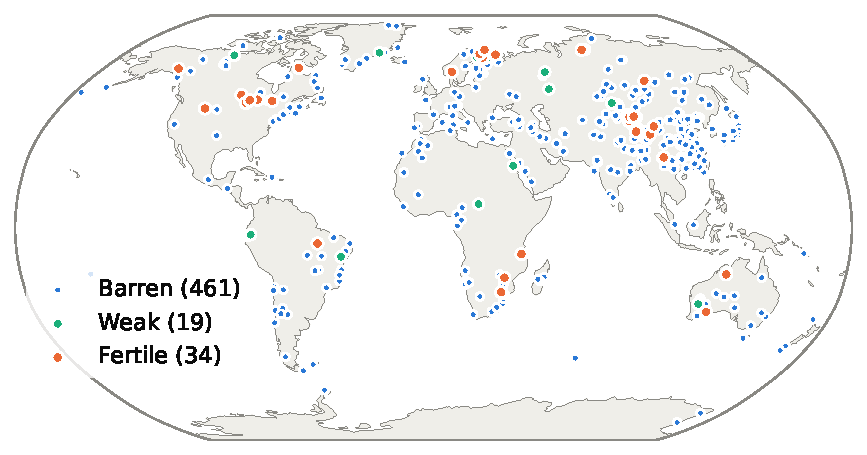
\includegraphics[width=0.86\textwidth]{figs/fig1_map.pdf}
\caption*{\textbf{Figure 1a.} Locations of the 514 benchmark intrusions with at least five GEOROC samples, colored by label: fertile (34), weakly mineralized (19) and barren (461). Robinson projection; coordinates are the median of each intrusion's sample coordinates.}
\vspace{6pt}
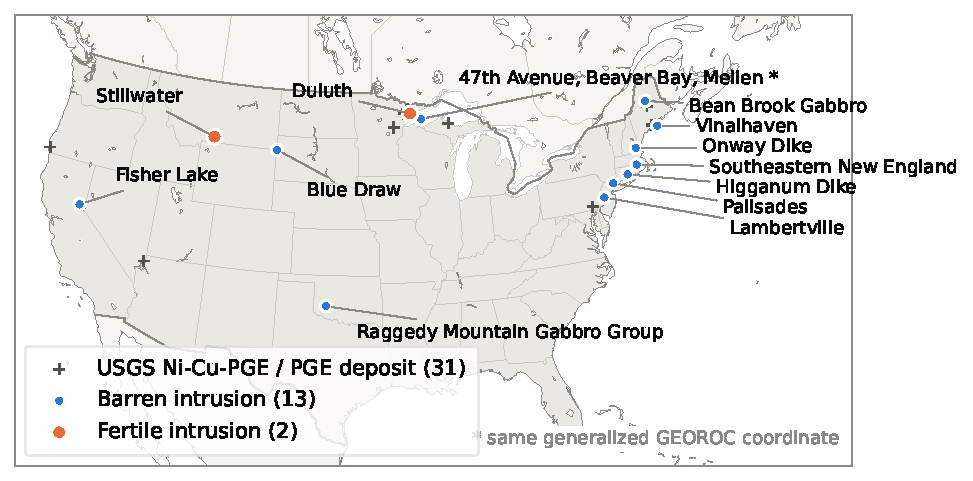
\includegraphics[width=0.86\textwidth]{figs/fig1b_map_conus.pdf}
\caption*{\textbf{Figure 1b.} Benchmark intrusions in the conterminous United States (15 intrusions: 2 fertile, 13 barren), shown with the 31 Ni-Cu-PGE and low-sulfide PGE deposits in the conterminous US listed in the USGS Critical Mineral Deposits database ver.~3.0 (crosses). 13 of these deposits, all outside the Stillwater and Duluth districts, lie more than 30~km from any benchmark sample (for example the Maine deposits, Tamarack and Eagle), so their host intrusions are not represented. Mellen, Beaver Bay and 47th Avenue share one generalized GEOROC coordinate (asterisk). Albers equal-area projection.}
\end{figure*}


A fundamental challenge, however, is that whole-rock compositions record not only the fertility of a magmatic system but also the petrologic context of individual samples \cite{behnsen2018,danso2026}. Chilled margins and fine-grained dikes may preserve compositions that approximate parental magmas entering an intrusion, whereas cumulates primarily record crystal accumulation and magmatic differentiation \cite{mungall2007,bai2019,holness2007}. Post-magmatic alteration may further modify major- and trace-element compositions \cite{danso2026,jackson2018}. As a result, a fertility index may distinguish among sample types or preservation states rather than between mineralized and barren systems. Comparisons that mix chilled margins, cumulates, differentiated rocks, and altered samples can therefore confound the geochemical signals of ore-forming processes with those of crystallization, accumulation, and alteration.

A second challenge is that published fertility indices were developed using different datasets, sampling strategies, analytical methods, and definitions of mineralization (e.g., \cite{nathwani2022,zou2022}) and therefore reported successes cannot be compared directly. An index calibrated on one group of intrusions may appear effective simply because of the samples included in the original study. This problem is analogous to model evaluation in machine learning, where meaningful comparison requires a common dataset, standardized labels, and a shared performance metric \cite{bender2022}. Without such a benchmark, it is difficult to determine whether differences among fertility indices reflect genuine predictive skill or differences in the underlying data used to develop them.

Here we present a curated benchmark dataset assembled from GEOROC 2.0 geochemical compilations \cite{lehnert2000,worner2024,digis2026} and the U.S. Geological Survey critical mineral deposits database \cite{hammarstrom2023}. GEOROC provides published whole-rock geochemical analyses and associated sample metadata, whereas the USGS database supplies independently documented information on mineralized systems. The benchmark is designed to evaluate how effectively published geochemical fertility indices distinguish intrusions hosting magmatic Ni-Cu-PGE sulfide mineralization from barren intrusions using a common set of samples, classifications, and scoring procedures. A central feature of the benchmark is explicit recognition of petrologic sample type. Each sample is classified as a chilled margin, fine-grained dike or sill, cumulate, altered, or unresolved. These labels allow fertility indices to be evaluated on comparable sample populations and make it possible to determine whether index performance varies systematically with sample type. An index evaluated on chilled-margin compositions may reflect processes operating in primitive magmas, whereas the same index applied to cumulates may primarily capture crystal accumulation or sulfide enrichment. Evaluating indices within defined petrologic groups therefore provides a more rigorous test of the geological processes that individual indices are intended to represent.

The benchmark is intended as an evaluation framework rather than a direct predictor of undiscovered mineral resources. Its results depend on the quality of published geochemical data, the completeness of sample metadata, the criteria used to define mineralization, and the distribution of available sample types across intrusions. However, by combining intrusion-level mineralization labels with sample-level petrologic classifications and an open scoring workflow, the benchmark provides a reproducible basis for evaluating existing geochemical fertility indices, identifying their limitations, and highlighting critical gaps in publicly available geochemical datasets. As a first application, we use the benchmark to compare published fertility indices within a common analytical framework and establish an initial performance leaderboard for open-data evaluation of magmatic Ni-Cu-PGE exploration criteria.

% =====================================================================
\section{Data and Methods}

\subsection{Data Sources}
Geochemical data were obtained from the GEOROC precompiled compilations \cite{digis2026} (DIGIS Team, September 2026 release), comprising ten tectonic-setting compilations distributed through GRO.data under a CC BY-SA 4.0 license (Table~A1). File fingerprints were recorded in the project provenance log to ensure reproducibility. The combined dataset contains 521,961 unique whole-rock analyses. The GEOROC Rock Types compilation was used as an independent completeness check. Information on mineralized systems was compiled from multiple sources, including the USGS Critical Mineral Deposits of the United States, version 3.0 \cite{hammarstrom2023}, the USGS magmatic Ni-Cu-PGE deposit inventory \cite{parks2026}, the USGS Mineral Resources Data System (MRDS) \cite{usgs2005}, and a curated literature database. After filtering to magmatic Ni and PGE occurrences, 665 MRDS records were retained for deposit classification.

\subsection{Sample Selection and Intrusion Assignment}
The initial compilation was filtered to plutonic mafic and ultramafic rocks using GEOROC lithological classifications. Retained rock types included gabbro, norite, troctolite, anorthosite, peridotite, dunite, pyroxenite, dolerite, picrite, cumulate rocks, and related lithologies. Samples associated with mantle xenoliths, kimberlite-hosted material, abyssal mantle, ophiolite complexes, orogenic peridotite massifs, and alkaline-carbonatite systems were excluded. The resulting dataset contained 31,886 samples (Table~A2).

Each sample was assigned to an intrusion using the GEOROC location hierarchy. Intrusion assignments were based on specific location level corresponding to an intrusion, layered complex, sill, chonolith, or equivalent igneous body. Where necessary, location comments were used to refine assignments. Samples lacking intrusion-level information and recorded only at a regional scale could not be assigned and were excluded from intrusion-based analyses. In total, 16,395 samples lacked sufficient geographic specificity for intrusion assignment. Intrusion names were standardized to remove spelling variations and synonymous forms using a manually curated alias table. Only intrusions represented by at least five samples were engaged in the benchmark dataset.

\subsection{Intrusion Mineralization Labels}

% ---------------- Figure 2 (sample types) ----------------
\begin{figure*}[t]
\centering
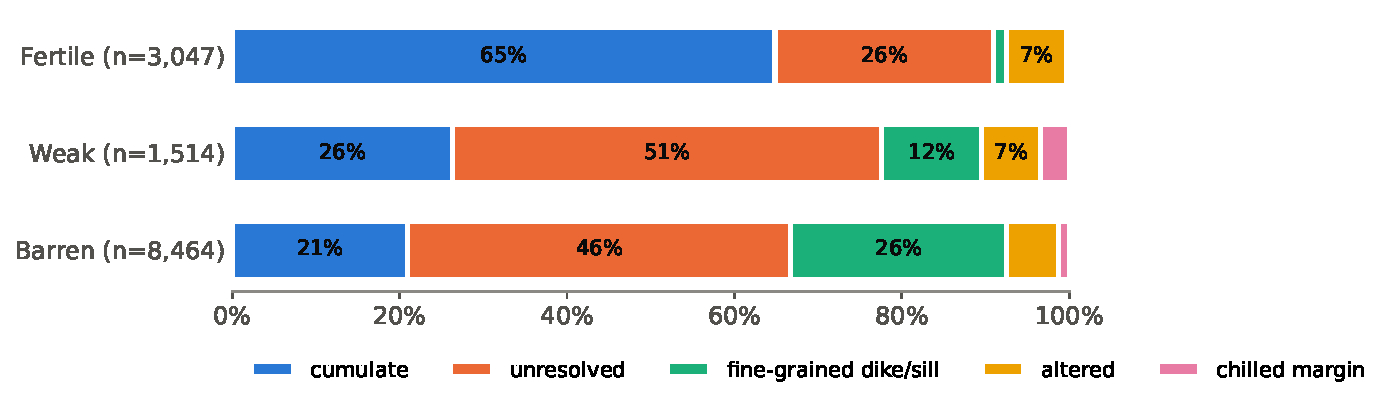
\includegraphics[width=0.92\textwidth]{figs/fig3_sample_types.pdf}
\caption*{\textbf{Figure 2.} Sample-type composition of fertile (\textit{n} = 3,047), weakly mineralized (\textit{n} = 1,514), and barren (\textit{n} = 8,464) intrusions. Bars show the percentage of samples in each category. Cumulate samples account for 65\% of samples from fertile intrusions, compared with 26\% from weakly mineralized and 21\% from barren intrusions. ``Unresolved'' indicates samples that could not be assigned to a specific type.}
\end{figure*}

Intrusions were classified into three mineralization categories: FERTILE: intrusions hosting a magmatic Ni-Cu-PGE sulfide deposit or reef-type PGE deposit with reported production or published mineral resources; WEAK: intrusions containing documented prospects or mineral occurrences but lacking established resources or production; BARREN: intrusions for which no evidence of magmatic Ni-Cu-PGE mineralization was identified. Initial classifications were generated using spatial and name-based matching against the USGS magmatic Ni-Cu-PGE inventory, USGS deposit databases, and MRDS records. Deposits or occurrences located within 10~km of intrusion sample locations were considered potential matches. MRDS producers were provisionally classified as FERTILE, whereas MRDS occurrences were classified as WEAK.

Because automated approaches provided uneven global coverage, particularly outside North America, intrusion classifications were subsequently reviewed against a curated literature compilation. Literature-based classifications were given precedence where conflicts existed. Every intrusion classified as FERTILE or WEAK is supported by at least one published source documenting mineralization (Supplementary Table~S1). Attention was given to cases where automated and literature-derived evidence disagreed. A total of 127 intrusions required manual review, including large intrusive complexes lacking deposit records and intrusions with conflicting classifications. Final automated and curated classifications differed for 66 intrusions, all of which are documented in the project repository. To acknowledge uncertainty in negative classifications, BARREN intrusions were assigned confidence levels. High-confidence barren classifications correspond to intrusions documented in the literature but associated only with other mineralization styles (e.g., Fe-Ti-V oxide or chromite deposits). Medium-confidence classifications correspond to reviewed intrusions located in regions with dense deposit coverage and reliable coordinate data. Remaining barren intrusions were assigned low confidence. The final benchmark contains 514 intrusions, including 34 FERTILE, 19 WEAK, and 461 BARREN systems, represented by 3,047, 1,514, and 8,464 samples, respectively (Table~A3).

\subsection{Sample-Type Classification}
To distinguish between petrologic contexts relevant to fertility assessment, each sample was assigned a single sample-type classification using a transparent hierarchy of reproducible rules. Five categories were recognized (Table~A4): (1) ALTERED: samples with loss-on-ignition (LOI) values greater than 5~wt.\%, moderate to extensive alteration recorded in GEOROC metadata, or alteration-related terminology in the sample description; (2) CHILLED\_MARGIN: samples described as chilled, quenched, marginal, or contact rocks; (3) CUMULATE: samples explicitly described as cumulates, exhibiting cumulate textures, composed of characteristic ultramafic or monomineralic cumulate lithologies, or containing $>$25~wt.\% MgO; (4) FINE\_GRAINED\_DIKE\_SILL: samples identified as dolerite, diabase, picrite, or associated with dike and sill units; (5) UNRESOLVED: samples that did not meet the criteria for the preceding categories.

The classification workflow records both the rule responsible for each assignment and whether the supporting evidence is considered strong or weak. Several quality-control procedures were applied prior to index calculation (Table~A7). A small number of PGE analyses were reported in inconsistent units in the original compilations. Following verification against the source publications, these values were converted to common units. MgO concentrations below 0.5~wt.\% were also excluded from all lithologies except anorthosite, where low MgO values are expected.

\subsection{Fertility Indices and Performance Evaluation}

% ---------------- Figure 3 (leaderboard) + Table 1 ----------------
\begin{figure*}[t]
\centering
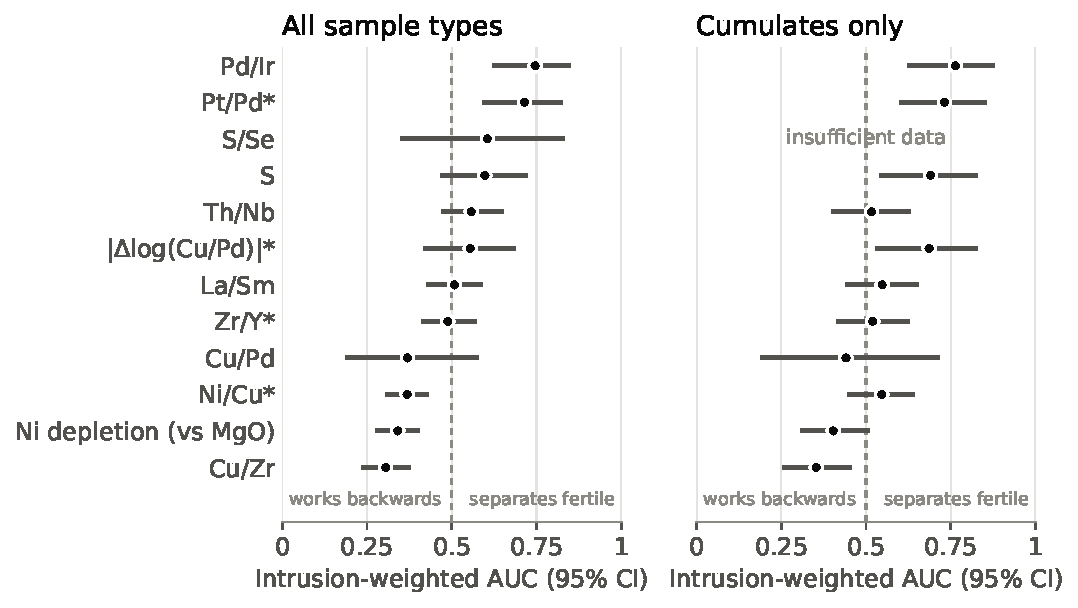
\includegraphics[width=0.84\textwidth]{figs/fig2_leaderboard.pdf}
\caption*{\textbf{Figure 3.} Leaderboard of the twelve fertility indices. Points show the intrusion-weighted ROC AUC and bars the 95\% confidence interval from 2,000 intrusion bootstrap resamples, for all sample types (left) and for cumulate samples only (right). Values above 0.5 (dashed line) mean the index ranks fertile intrusions above barren ones; values below 0.5 mean it ranks barren intrusions above fertile ones (``works backwards''). Asterisks mark the four exploratory indices defined for this study. ``Insufficient data'': fewer than five fertile or five barren intrusions had data for the index.}
\end{figure*}

\begin{table*}[t]
\caption*{\textbf{Table 1.} Leaderboard: intrusion-weighted ROC AUC (95\% bootstrap confidence interval) for each index, for all samples and by sample type. ``--'' marks subsets with fewer than five fertile or five barren intrusions. Coverage is the share of benchmark samples with the elements the index needs. Asterisks mark exploratory indices.}
\centering\footnotesize
\setlength{\tabcolsep}{4pt}
\begin{tabular}{@{}lccccccc@{}}
\toprule
Index & All samples & Cumulates & \begin{tabular}[c]{@{}c@{}}Chilled margins +\\ dikes/sills\end{tabular} & Altered & Unresolved & \begin{tabular}[c]{@{}c@{}}Fertile / barren\\ intrusions\end{tabular} & Coverage \\
\midrule
\tabinput{tab_leaderboard.tex}
\bottomrule
\end{tabular}
\end{table*}

Twelve fertility indices were evaluated (Table~A5). Eight correspond to previously published geochemical indicators of magmatic sulfide fertility, whereas four represent exploratory variants developed for this study. All indices were implemented programmatically to ensure consistent calculation and reproducibility. Published indices were oriented according to the fertility hypotheses proposed in their original studies. Exploratory indices, including a two-sided Cu/Pd deviation from primitive mantle, Pt/Pd, Ni/Cu, and Zr/Y, were assigned directional interpretations prior to evaluation. Ratio-based indices were log-transformed before scoring. Nickel depletion was quantified as the negative residual from a label-independent quadratic regression of log(Ni) versus MgO fitted across the entire dataset. Primitive mantle normalizations followed the values of McDonough and Sun \cite{mcdonough1995}.

Index performance was assessed using the area under the receiver operating characteristic curve (ROC AUC) for discrimination between FERTILE and BARREN intrusions. WEAK intrusions were excluded from performance calculations. To prevent heavily sampled intrusions from dominating results, each sample received a weight equal to the inverse of the number of samples assigned to its intrusion, thereby giving all intrusions equal influence on the final score \cite{fawcett2006}. Uncertainty was estimated using 2,000 bootstrap resamples of intrusions within each mineralization class. Reported confidence intervals correspond to the 95\% bootstrap percentile range. An AUC value greater than 0.5 indicates that an index preferentially ranks fertile intrusions above barren intrusions, whereas values below 0.5 indicate the opposite relationship. Scores were calculated for the complete dataset and separately for each sample-type category. To ensure meaningful evaluation, a sample-type subset was scored only when at least five fertile and five barren intrusions contained valid data. For methods requiring parameter estimation or model fitting, performance was evaluated using a fixed holdout set comprising 30\% of intrusions, reserved prior to model development and excluded from parameter tuning.


% =====================================================================
\section{Results}

\subsection{Benchmark Composition and Sample Distribution}

% ---------------- Figure 4 ----------------
\begin{figure*}[t]
\centering
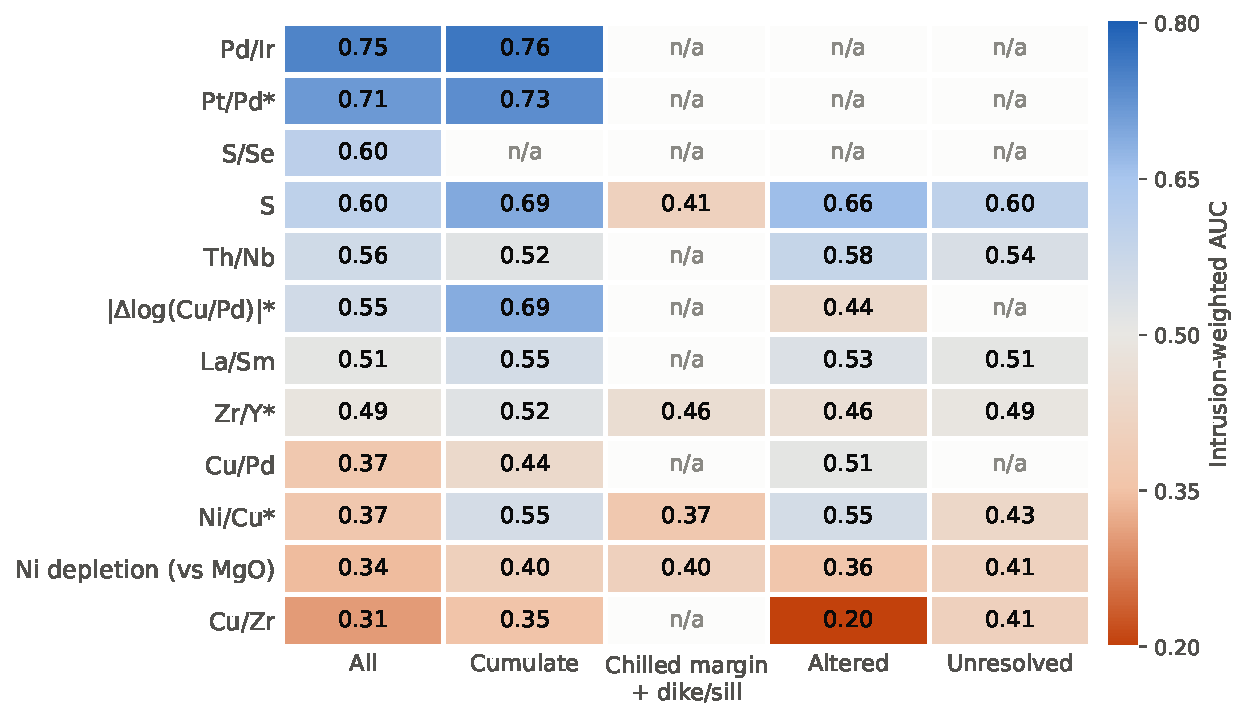
\includegraphics[width=0.78\textwidth]{figs/fig4_auc_by_sample_type.pdf}
\caption*{\textbf{Figure 4.} Intrusion-weighted area under the receiver operating characteristic curve (AUC) for each geochemical index, calculated using all samples and the indicated sample types. Cells are marked ``n/a'' where fewer than five fertile or five barren intrusions had data for that index and sample type. The diverging color scale is centered at AUC = 0.5; asterisks denote the same conditions as in Figure~3.}
\end{figure*}

The final benchmark comprises 13,025 samples from 514 named mafic-ultramafic intrusions distributed across all major continents (Fig.~1a). The dataset includes 34 FERTILE, 19 WEAK, and 461 BARREN intrusions, represented by 3,047, 1,514, and 8,464 samples, respectively. The geographic distribution of benchmark intrusions spans Archean cratons, continental rifts, large igneous provinces, layered intrusions, and arc-related magmatic systems, providing a globally distributed test set for evaluating fertility indices. 13 of the 31 continental USA deposits lie more than 30~km from any benchmark sample (Fig.~1b). These are the five Maine deposits, the four Tamarack zones, Eagle deposit, Gap (Pennsylvania), Red Flats (Oregon) and Key West (Nevada), so their host intrusions aren't represented in GEOROC. The remaining 18 are in the Stillwater and Duluth districts, which do have samples.

Sample-type distributions vary markedly among mineralization classes (Fig.~2). Fertile intrusions are strongly dominated by cumulate rocks, which constitute approximately 65\% (1,976/3,047) of all fertile samples. In contrast, cumulates account for only 21\% of samples from barren intrusions. Barren intrusions contain substantially higher proportions of fine-grained dike and sill samples (26\%) and unresolved lithologies (46\%) than fertile intrusions. Altered samples comprise a relatively small proportion of each class, ranging from approximately 6--7\%. The benchmark also reveals imbalance in the availability of parental magma proxies. Chilled-margin samples are rare throughout the dataset, and only ten fertile intrusions contain any chilled-margin or fine-grained dike/sill samples. The benchmark is dominated by cumulate lithologies from fertile systems rather than by magma compositions that directly record intrusion emplacement. This imbalance has important implications for the interpretation of fertility indices because many published indices were originally developed to evaluate parental magma signatures rather than cumulate rocks.



\subsection{Performance of Published Fertility Indices}
Index performance was evaluated using intrusion-weighted receiver operating characteristic area under the curve (ROC AUC) values, with confidence intervals generated by bootstrap resampling (Table~1; Fig.~3). Across all sample types, Pd/Ir achieved the highest discrimination between fertile and barren intrusions, yielding an intrusion-weighted AUC of 0.75 (95\% CI: 0.62--0.85). The exploratory Pt/Pd metric ranked second with an AUC of 0.71 (95\% CI: 0.59--0.83). These were the only indices whose confidence intervals remained entirely above 0.5, indicating statistically robust discrimination of fertile and barren intrusions within the benchmark. Indices based on sulfur abundance and sulfur behavior showed intermediate performance. Both S/Se and S achieved AUC values of approximately 0.60, suggesting modest but positive discrimination. Indices intended to capture crustal contamination yielded values close to random classification. Th/Nb produced an AUC of 0.56, La/Sm yielded 0.51, and Zr/Y yielded 0.49, indicating only weak separation of fertile and barren systems.

Some important fertility metrics performed substantially worse than random expectation. Ni/Cu, Ni depletion relative to MgO, and Cu/Zr produced AUC values of 0.37, 0.34, and 0.31, respectively. The confidence intervals for these indices remained entirely below 0.5, indicating that they systematically ranked barren intrusions ahead of fertile intrusions in the benchmark dataset. Cu/Pd also yielded an AUC of 0.37, but its confidence interval (0.19--0.58) includes 0.5. Rather than reflecting an absence of signal, these results imply that the direction of association predicted by the original fertility hypotheses is reversed in the compiled sample population. Overall, the leaderboard is dominated by PGE-based metrics, whereas contamination-based and depletion-based indices provide limited discrimination between fertile and barren intrusions (Table~1; Fig.~3).

\subsection{Influence of Sample Type on Index Performance}
The effectiveness of fertility indices varies considerably with sample type (Figs.~3 and 4; Table~1). Restricting analysis to cumulate samples generally improved performance for many indices. Among cumulates, Pd/Ir increased slightly from 0.75 to 0.76, while Pt/Pd increased from 0.71 to 0.73. Sulfur concentration showed one of the largest improvements, increasing from 0.60 in the complete dataset to 0.69 in cumulates. Several indices that performed poorly in the full dataset showed notable improvement when evaluated only on cumulates. For example, the exploratory $|\Delta\log(\mathrm{Cu/Pd})|$ metric increased from 0.55 to 0.69, and Ni/Cu increased from 0.37 to 0.55. Although these indices remained weaker than Pd/Ir and Pt/Pd, the magnitude of the improvement demonstrates that lithologic mixing can substantially influence observed assay performance.


Performance within altered samples differed markedly from that observed in cumulates. In some cases, discrimination weakened substantially. For example, Cu/Zr decreased to an AUC of 0.20 in altered rocks, while Ni depletion remained consistently below random expectation across most sample classes. These results indicate that alteration and sample context can substantially modify the behavior of fertility indicators originally developed for relatively fresh magmatic rocks. The scarcity of chilled-margin samples prevented stout evaluation of most indices in compositions interpreted to approximate parental magmas. Only a small subset of indices met the minimum data requirements for chilled-margin and fine-grained dike/sill categories, and confidence intervals remained correspondingly broad. The current benchmark provides a much stronger assessment of index performance in cumulates than in parental magma compositions.

\subsection{Sensitivity Analysis}
To evaluate the effect of uncertainty in barren classifications, the analysis was repeated using only MEDIUM- and HIGH-confidence barren intrusions. Restricting the benchmark in this manner produced only modest changes in leaderboard rankings. The highest-performing index, Pd/Ir, declined from an AUC of 0.75 to 0.71, while retaining its position as the best-performing metric. The limited change observed during sensitivity testing suggests that the principal conclusions of the benchmark are robust to reasonable variations in barren-intrusion classification. Complete sensitivity-analysis results for all indices are provided in the accompanying data release (Table~A6).

\subsection{Label Verification and Quality Control}
Benchmark construction included manual review of intrusion classifications and automated sample assignments. The authors reviewed 127 intrusion labels where automated and literature-derived evidence conflicted or where known mineralized systems lacked supporting database records. Each reviewed intrusion was either confirmed or reassigned based on published deposit documentation, and all final decisions are archived with the benchmark dataset. As an additional quality-control measure, eleven named and randomly selected samples were traced back to their original GEOROC records. In every case, benchmark values matched the source compilation, indicating that sample extraction and processing were performed correctly.

Sample-type classifications were subjected to preliminary spot checks, but a systematic expert review has not yet been completed. No quantitative agreement statistic between rule-based and expert classifications is reported in the present version of the benchmark. The current sample-type tags should therefore be regarded as provisional. A formal validation exercise comparing rule-based classifications with expert interpretations is planned for version 0.2 of the benchmark and will provide an independent assessment of classification accuracy.

% =====================================================================
\section{Discussion}

The benchmark highlights a fundamental challenge in evaluating geochemical fertility indices: many indices were developed to diagnose specific stages of the magmatic sulfide-forming process, yet compiled datasets often contain samples that represent very different petrologic contexts. As a result, index performance reflects not only the validity of the underlying geochemical model, but also whether the sampled rocks preserve the geological signal that the index was designed to detect. Three of the poorest-performing indices in the benchmark, Cu/Zr, Ni depletion relative to MgO, and Cu/Pd, illustrate this problem clearly. These indices were developed to identify magmas that have lost chalcophile metals to an immiscible sulfide liquid. In their intended setting, sulfide segregation removes Cu, Ni, and PGE from the silicate melt, producing geochemical depletion signatures in residual liquids \cite{mansur2021,pina2013}. Such signatures are most appropriately evaluated in rocks that approximate magma compositions, including chilled margins and fine-grained feeder dikes. However, when applied to cumulates containing accumulated sulfide minerals, the expected relationships are reversed. High Cu relative to Zr, elevated Ni at a given MgO content, and low Cu/Pd ratios can reflect sulfide accumulation rather than sulfide depletion \cite{gao2012,gao2013,seat2009}. Indices designed to identify depleted melts may systematically rank sulfide-rich cumulates as fertile when interpreted in reverse or rank barren systems ahead of fertile systems when applied without regard to sample type \cite{grondahl2021,grondahlzajacz2022}.

The benchmark demonstrates this effect at a global scale. Fertile intrusions in the dataset are represented by cumulate rocks, which constitute 65\% of all fertile samples, whereas chilled margins and fine-grained dike or sill samples are rare. The poor performance of depletion-based indices therefore does not necessarily invalidate the geological concepts underlying those indices. Rather, it indicates a mismatch between the sample types for which the indices were developed and the sample types that dominate available open geochemical compilations. This result emphasizes a long-recognized principle in magmatic sulfide exploration: depletion indices should be evaluated primarily on rocks that preserve liquid compositions rather than on rocks dominated by crystal accumulation and sulfide concentration \cite{barnes2023,barneswilliams2024}. In contrast, the strongest-performing indices in the benchmark are based on platinum-group element ratios. Pd/Ir achieved the highest intrusion-weighted AUC, followed by Pt/Pd, and both remained effective when restricted to cumulates. This result suggests that PGE-ratio indices may capture features of ore-forming systems that are less sensitive to the distinction between liquid and cumulate compositions \cite{barneswilliams2024,grondahlzajacz2022}. These results should be interpreted cautiously, only a limited number of fertile intrusions contain the PGE analyses required for calculating these ratios, resulting in relatively broad confidence intervals. Additional PGE data from both mineralized and barren intrusions will be required to determine whether the observed ranking remains stable as benchmark coverage expands.

Perhaps the most important outcome of this study is not the leaderboard itself, but the identification of a major gap in publicly available geochemical datasets. Despite decades of research on magmatic sulfide systems, chilled-margin and feeder-dike samples from known ore-bearing intrusions remain underrepresented in open geochemical repositories. Many published fertility indices cannot yet be subjected to a rigorous large-scale test using the sample types for which they were originally intended. The current benchmark therefore provides a stronger evaluation of fertility indices in cumulate-rich datasets than in parental magma compositions. The benchmark also highlights opportunities for community-driven improvement. The most valuable contribution would be the addition of whole-rock analyses from chilled margins, feeder dikes, and sulfide-poor marginal lithologies of well-characterized mineralized intrusions. Such samples are critical for testing hypotheses related to magma fertility, sulfide saturation, and metal depletion. A second priority is improving the quality of barren intrusion labels through the documentation of explored but demonstrably unmineralized systems. Improved characterization of negative examples would reduce uncertainty in benchmark classifications and strengthen future comparisons among competing fertility metrics.

Because the benchmark framework separates data, labels, and scoring procedures, these improvements can be incorporated without modifying the underlying evaluation methodology. As additional geochemical analyses and deposit information become available, the benchmark can be expanded and updated while preserving direct comparability with previous results. In this sense, the present study should be viewed as a first iteration of an evolving community resource for evaluating geochemical indicators of magmatic Ni-Cu-PGE fertility.

% =====================================================================
\section{Limitations}

The benchmark has several important limitations. Intrusion labels rely partly on a curated literature compilation, and many barren classifications indicate only that no Ni-Cu-PGE deposit is currently recorded rather than demonstrating that an intrusion is truly unmineralized. Approximately half of the mafic-ultramafic samples identified in GEOROC could not be confidently assigned to a named intrusion and were therefore excluded from benchmarking. Sample-type classifications are based on transparent rule-based criteria and have not yet been systematically validated against expert interpretations. The benchmark also inherits variable data quality, metadata completeness, and reporting standards from the underlying GEOROC sources, and a small number of records required unit or value corrections during quality control. ROC AUC evaluates the relative ranking ability of an index but does not define practical exploration cutoffs or directly measure exploration success. The benchmark should be viewed as a comparative framework for evaluating fertility indices rather than a predictor of undiscovered mineral resources.

% =====================================================================
\section*{\textit{Use of AI Tools}}
\textit{The authors used an artificial intelligence assistant to assist with the development of data-processing and analysis pipeline code. The authors made all methodological and analytical decisions, curated and reviewed intrusion labels and sample-type classifications, verified data corrections against original sources, interpreted the results, and wrote and revised the manuscript. The authors take full responsibility for the accuracy, interpretation, and content of the work.}

\section*{Author Contributions (CRediT)}
Danso Bezali K.: Conceptualization, methodology, data curation, software, formal analysis, validation, investigation, visualization, manuscript writing -- original draft. Dankwa Josephine O.: Review \& editing of the manuscript. Aidoo Adwoa A.: Review and editing (methodology and conceptualization).

\section*{Data Availability}
The benchmark data, curated intrusion labels, scoring program, leaderboard, figures and tables (release v0.1.0) are archived on Zenodo at \doi{10.5281/zenodo.23777406} and maintained at \url{https://github.com/bkdanso/fertile-or-barren}. Data are released under CC BY-SA 4.0, as required by GEOROC, and code under the MIT license. All tables, including the full list of 514 benchmark intrusions (Table~S2), are provided in Supplementary file S1.

\section*{Competing Interests}
The authors declare no competing interests.

\section*{Funding}
This research received no external funding.

\section*{Supplementary Materials}
Table S1. Deposit and occurrence references supporting all intrusion-level fertility classifications are provided in \textit{intrusion\_labels\_curated.csv}. Each intrusion classified as FERTILE or WEAK is linked to one or more published references documenting the associated deposit, occurrence, or prospect. Table~S1 is reproduced in Appendix~B.

% =====================================================================
\onecolumn
\appendix
\renewcommand{\thetable}{A\arabic{table}}
\setcounter{table}{0}
\captionsetup[table]{name=Table}
\section*{Appendix A. Benchmark Construction Tables}

\begin{table}[h]
\caption{Data sources.}
\centering\small
\begin{tabularx}{\textwidth}{@{}>{\raggedright}p{4.2cm}>{\raggedright}p{2.6cm}>{\raggedright}p{2.3cm}>{\raggedright}X>{\raggedright}p{1.6cm}>{\raggedright\arraybackslash}p{3.2cm}@{}}
\toprule
Source & Producer & Version & Records used & License & Identifier \\
\midrule
GEOROC precompiled compilations (10 tectonic-setting compilations) \cite{digis2026} & DIGIS Team, GRO.data & September 2026 (v13.0) & 521,961 unique analyses (whole-rock geochemistry) & CC BY-SA 4.0 & \doi{10.25625/1KRR1P} and 9 others \\
GEOROC Compilation: Rock Types (mafic-ultramafic files) \cite{digis2026} & DIGIS Team, GRO.data & September 2026 (v15.0) & Completeness cross-check: 31,222 plutonic analyses; 160 absent from the union & CC BY-SA 4.0 & \doi{10.25625/2JETOA} \\
Critical Mineral Deposits of the United States \cite{hammarstrom2023} & USGS & ver.~3.0, September 2026 & 37 Ni-Cu-PGE / PGE deposits (US deposit locations) & CC0 & \doi{10.5066/P9K1HBNT} \\
Magmatic Ni-Cu-PGE inventory \cite{parks2026} & USGS & 2026 & Host intrusions and resources (US); intrusion names matched & CC0 & \doi{10.5066/P1YLGLUZ} \\
Mineral Resources Data System (MRDS) \cite{usgs2005} & USGS & Full CSV export & 665 magmatic Ni or PGE records (global deposit and occurrence locations) & Public domain & \url{https://mrdata.usgs.gov/mrds/} \\
\bottomrule
\end{tabularx}
\end{table}

\begin{table}[h]
\begin{minipage}[t]{0.5\textwidth}
\caption{Sample selection, from GEOROC rows to the benchmark.}
\centering\footnotesize
\begin{tabular}{@{}lr@{}}
\toprule
Stage & Count \\
\midrule
\tabinput{tab_selection.tex}
\bottomrule
\end{tabular}
\end{minipage}\hfill
\begin{minipage}[t]{0.44\textwidth}
\caption{Intrusion labels by confidence level.}
\centering\small
\begin{tabular}{@{}llrr@{}}
\toprule
Label & Confidence & Intrusions & Samples \\
\midrule
\tabinput{tab_labels.tex}
\midrule
Total & & 514 & 13,025 \\
\bottomrule
\end{tabular}
\end{minipage}
\end{table}

\begin{table}[h]
\caption{Sample types by label: number of samples (share of the label's samples; number of intrusions with at least one sample of that type).}
\centering\small
\setlength{\tabcolsep}{4pt}
\begin{tabular}{@{}lcccccr@{}}
\toprule
Label & Cumulate & Unresolved & Fine-grained dike/sill & Altered & Chilled margin & Total samples \\
\midrule
\tabinput{tab_types.tex}
\bottomrule
\end{tabular}
\end{table}

\begin{table}[h]
\caption{Index definitions. Each score is oriented so that a higher value means ``predicted fertile''. Asterisks mark exploratory indices whose direction was set by the authors before scoring. PM: primitive mantle \cite{mcdonough1995}.}
\centering\footnotesize
\begin{tabularx}{\textwidth}{@{}>{\raggedright}p{2.5cm}>{\raggedright}p{2.6cm}>{\raggedright}p{4.0cm}>{\raggedright}X>{\raggedright\arraybackslash}p{1.6cm}@{}}
\toprule
Index & Family & Score & Hypothesis tested & Reference \\
\midrule
Cu/Pd & Chalcophile ratio & $\log_{10}$(Cu/Pd) & High Cu/Pd (above mantle) = PGE stripped by earlier sulfide = fertile & \cite{barnes1993,li2001} \\
$|\Delta\log(\mathrm{Cu/Pd})|$* & Chalcophile ratio (exploratory) & $|\log_{10}(\mathrm{Cu/Pd}) - \log_{10}(\mathrm{Cu/Pd})_{\mathrm{PM}}|$ & Any departure of Cu/Pd from mantle (high = depleted, low = sulfide-enriched) = sulfide involvement & this study; \cite{mcdonough1995} \\
Pd/Ir & Chalcophile ratio & $\log_{10}$(Pd/Ir) & High Pd/Ir = fractionated, sulfide-associated PGE signature = fertile & \cite{barnes1985} \\
Pt/Pd* & Chalcophile ratio (exploratory) & $-\log_{10}$(Pt/Pd) & Low Pt/Pd = Pd-rich, sulfide-associated PGE = fertile & this study \\
Cu/Zr & Chalcophile ratio & $-\log_{10}$(Cu/Zr) & Low Cu/Zr = Cu depleted relative to an incompatible element = sulfide removed = fertile & \cite{lightfoot1990} \\
Ni/Cu* & Chalcophile ratio (exploratory) & $-\log_{10}$(Ni/Cu) & Low Ni/Cu = Cu-rich, sulfide-fractionated signature & this study \\
Ni depletion (vs MgO) & Ni depletion & $-(\log_{10}\mathrm{Ni} - $ quadratic fit of $\log_{10}$Ni on MgO, 5--50 wt\%) & Ni below the olivine-controlled Ni-MgO trend = Ni lost to sulfide = fertile & \cite{linaldrett1999,barneslightfoot2005} \\
Th/Nb & Crustal contamination & $\log_{10}$(Th/Nb) & High Th/Nb = crustal contamination, a common trigger of sulfide saturation = fertile & \cite{lightfoot1993,pearce2008} \\
La/Sm & Crustal contamination & $\log_{10}$(La/Sm) & High La/Sm = LREE enrichment from crustal contamination = fertile & \cite{lightfoot1990} \\
Zr/Y* & Crustal contamination (exploratory) & $\log_{10}$(Zr/Y) & High Zr/Y = enriched or contaminated source & this study \\
S & Sulfur & $\log_{10}$(S) & High whole-rock S = sulfide present = fertile & \cite{barneslightfoot2005} \\
S/Se & Sulfur & $\log_{10}$(S/Se) & S/Se above mantle range = external crustal S added = fertile & \cite{queffurus2015} \\
\bottomrule
\end{tabularx}
\end{table}

\begin{table}[h]

\caption{Robustness of the intrusion-weighted AUC. ``--'': not enough intrusions in the subset.}
\centering\small
\setlength{\tabcolsep}{3.5pt}
\begin{tabular}{@{}lcccc@{}}
\toprule
Index & \begin{tabular}[c]{@{}c@{}}AUC$_w$\\(all)\end{tabular} & \begin{tabular}[c]{@{}c@{}}AUC on\\intrusion medians\end{tabular} & \begin{tabular}[c]{@{}c@{}}AUC$_w$, LOW-conf.\\barren removed\end{tabular} & \begin{tabular}[c]{@{}c@{}}AUC$_w$, test split\\(30\% of intrusions)\end{tabular} \\
\midrule
\tabinput{tab_robust.tex}
\bottomrule
\end{tabular}
\end{table}

\begin{table}[h]
\caption{Data corrections applied before scoring.}
\centering\footnotesize
\begin{tabular}{@{}>{\raggedright}p{3cm}>{\raggedright}p{7.5cm}r>{\raggedright\arraybackslash}p{4.6cm}@{}}
\toprule
Correction & Rule & Samples & Note \\
\midrule
\tabinput{tab_corr.tex}
\bottomrule
\end{tabular}
\end{table}

\clearpage
\section*{Appendix B. Table S1: Fertile and Weakly Mineralized Intrusions}
{\footnotesize
\setlength{\tabcolsep}{4pt}
\begin{longtable}{@{}>{\raggedright}p{2.9cm}cr>{\raggedright}p{6.2cm}>{\raggedright}p{3.3cm}>{\raggedright\arraybackslash}p{1.4cm}@{}}
\caption*{\small\textbf{Table S1.} The 53 intrusions labeled FERTILE (F) or WEAK (W), with the deposit or occurrence and the published source supporting the label. \textit{n}: benchmark samples. The 461 BARREN intrusions are listed in Table S2 (Supplementary file S1 and Zenodo record).}\\
\toprule
Intrusion & Label & \textit{n} & Deposit / occurrence & Deposit type & Reference \\
\midrule
\endfirsthead
\toprule
Intrusion & Label & \textit{n} & Deposit / occurrence & Deposit type & Reference \\
\midrule
\endhead
\bottomrule
\endfoot
\tabinput{tab_s1.tex}
\end{longtable}}

% =====================================================================
\twocolumn
\section*{References}
\begingroup
\renewcommand{\section}[2]{}
\begin{thebibliography}{99}

\bibitem{mudd2014} G. M. Mudd and S. M. Jowitt. A detailed assessment of global nickel resource trends and endowments. \textit{Econ. Geol.}, 109(7):1813--1841, 2014. \doi{10.2113/econgeo.109.7.1813}.

\bibitem{naldrett2004} A. J. Naldrett. \textit{Magmatic Sulfide Deposits: Geology, Geochemistry and Exploration}. Springer, Berlin, 2004. \doi{10.1007/978-3-662-08444-1}.

\bibitem{barneslightfoot2005} S.-J. Barnes and P. C. Lightfoot. Formation of magmatic nickel sulfide deposits and processes affecting their copper and platinum-group element contents. In \textit{Economic Geology 100th Anniversary Volume}, pages 179--213. Society of Economic Geologists, 2005. \doi{10.5382/AV100.08}.

\bibitem{naldrett2010} A. J. Naldrett. Secular variation of magmatic sulfide deposits and their source magmas. \textit{Econ. Geol.}, 105(3):669--688, 2010. \doi{10.2113/gsecongeo.105.3.669}.

\bibitem{barnes1985} S.-J. Barnes, A. J. Naldrett, and M. P. Gorton. The origin of the fractionation of platinum-group elements in terrestrial magmas. \textit{Chem. Geol.}, 53(3--4):303--323, 1985. \doi{10.1016/0009-2541(85)90076-2}.

\bibitem{barnes1993} S.-J. Barnes, J.-F. Couture, E. W. Sawyer, and C. Bouchaib. Nickel-copper occurrences in the Belleterre-Angliers Belt of the Pontiac Subprovince and the use of Cu-Pd ratios in interpreting platinum-group element distributions. \textit{Econ. Geol.}, 88(6):1402--1418, 1993. \doi{10.2113/gsecongeo.88.6.1402}.

\bibitem{queffurus2015} M. Queffurus and S.-J. Barnes. A review of sulfur to selenium ratios in magmatic nickel-copper and platinum-group element deposits. \textit{Ore Geol. Rev.}, 69:301--324, 2015. \doi{10.1016/j.oregeorev.2015.02.019}.

\bibitem{lightfoot1990} P. C. Lightfoot, A. J. Naldrett, N. S. Gorbachev, W. Doherty, and V. A. Fedorenko. Geochemistry of the Siberian Trap of the Noril'sk area, USSR, with implications for the relative contributions of crust and mantle to flood basalt magmatism. \textit{Contrib. Mineral. Petrol.}, 104(6):631--644, 1990. \doi{10.1007/BF01167284}.

\bibitem{lightfoot1993} P. C. Lightfoot, C. J. Hawkesworth, J. Hergt, A. J. Naldrett, N. S. Gorbachev, V. A. Fedorenko, and W. Doherty. Remobilisation of the continental lithosphere by a mantle plume: major-, trace-element, and Sr-, Nd-, and Pb-isotope evidence from picritic and tholeiitic lavas of the Noril'sk District, Siberian Trap, Russia. \textit{Contrib. Mineral. Petrol.}, 114(2):171--188, 1993. \doi{10.1007/BF00307754}.

\bibitem{linaldrett1999} C. Li and A. J. Naldrett. Geology and petrology of the Voisey's Bay intrusion: reaction of olivine with sulfide and silicate liquids. \textit{Lithos}, 47(1--2):1--31, 1999. \doi{10.1016/S0024-4937(99)00005-5}.

\bibitem{li2001} C. Li, W. D. Maier, and S. A. de Waal. Magmatic Ni-Cu versus PGE deposits: contrasting genetic controls and exploration implications. \textit{S. Afr. J. Geol.}, 104(4):309--318, 2001. \doi{10.2113/gssajg.104.4.309}.

\bibitem{pearce2008} J. A. Pearce. Geochemical fingerprinting of oceanic basalts with applications to ophiolite classification and the search for Archean oceanic crust. \textit{Lithos}, 100(1--4):14--48, 2008. \doi{10.1016/j.lithos.2007.06.016}.

\bibitem{behnsen2018} H. Behnsen. \textit{Magma fertility related to Au-Cu mineralisation: evaluating the potential for linked porphyry Cu-Au deposits at depths, North Queensland, Australia}. PhD thesis, James Cook University, 2018.

\bibitem{danso2026} B. K. Danso and S. Abdullah. MCR-GeoChem v1.0.1: harmonized whole-rock and mineral geochemistry of the Midcontinent Rift (Michigan, Minnesota, Wisconsin). \textit{Zenodo}, 2026. \doi{10.5281/zenodo.23516434}.

\bibitem{mungall2007} J. E. Mungall. Crustal contamination of picritic magmas during transport through dikes: the Expo Intrusive Suite, Cape Smith fold belt, New Quebec. \textit{J. Petrol.}, 48(5):1021--1039, 2007. \doi{10.1093/petrology/egm009}.

\bibitem{bai2019} Z. J. Bai, H. Zhong, R. Z. Hu, W. G. Zhu, and W. J. Hu. Composition of the chilled marginal rocks of the Panzhihua layered intrusion, Emeishan Large Igneous Province, SW China: implications for parental magma compositions, sulfide saturation history and Fe-Ti oxide mineralization. \textit{J. Petrol.}, 60(3):619--648, 2019. \doi{10.1093/petrology/egz008}.

\bibitem{holness2007} M. B. Holness, M. A. Hallworth, A. Woods, and R. E. Sides. Infiltration metasomatism of cumulates by intrusive magma replenishment: the Wavy Horizon, Isle of Rum, Scotland. \textit{J. Petrol.}, 48(3):563--587, 2007. \doi{10.1093/petrology/egl072}.

\bibitem{jackson2018} M. D. Jackson, J. Blundy, and R. S. J. Sparks. Chemical differentiation, cold storage and remobilization of magma in the Earth's crust. \textit{Nature}, 564(7736):405--409, 2018. \doi{10.1038/s41586-018-0746-2}.

\bibitem{nathwani2022} C. L. Nathwani, J. J. Wilkinson, G. Fry, R. N. Armstrong, D. J. Smith, and C. Ihlenfeld. Machine learning for geochemical exploration: classifying metallogenic fertility in arc magmas and insights into porphyry copper deposit formation. \textit{Miner. Deposita}, 57(7):1143--1166, 2022. \doi{10.1007/s00126-021-01086-9}.

\bibitem{zou2022} S. Zou, X. Chen, M. J. Brzozowski, C. B. Leng, and D. Xu. Application of machine learning to characterizing magma fertility in porphyry Cu deposits. \textit{J. Geophys. Res. Solid Earth}, 127(8):e2022JB024584, 2022. \doi{10.1029/2022JB024584}.

\bibitem{bender2022} A. Bender, N. Schneider, M. Segler, W. Patrick Walters, O. Engkvist, and T. Rodrigues. Evaluation guidelines for machine learning tools in the chemical sciences. \textit{Nat. Rev. Chem.}, 6(6):428--442, 2022. \doi{10.1038/s41570-022-00391-9}.

\bibitem{lehnert2000} K. Lehnert, Y. Su, C. H. Langmuir, B. Sarbas, and U. Nohl. A global geochemical database structure for rocks. \textit{Geochem. Geophys. Geosyst.}, 1(5):1999GC000026, 2000. \doi{10.1029/1999GC000026}.

\bibitem{worner2024} G. Wörner et al. GEOROC 2.0: a globally connected geochemical database to facilitate interdisciplinary, data-driven research. \textit{EGU General Assembly 2024}, EGU24-15541, 2024. \doi{10.5194/egusphere-egu24-15541}.

\bibitem{digis2026} DIGIS Team. GEOROC Compilations (Archaean Cratons; Complex Volcanic Settings; Continental Flood Basalts; Convergent Margins; Intraplate Volcanic Rocks; Ocean Basin Flood Basalts; Ocean Island Groups; Oceanic Plateaus; Rift Volcanics; Seamounts; Rock Types). \textit{GRO.data}, v13.0 (Rock Types v15.0), 2026. \doi{10.25625/1KRR1P}; \doi{10.25625/1VOFM5}; \doi{10.25625/WSTPOX}; \doi{10.25625/PVFZCE}; \doi{10.25625/RZZ9VM}; \doi{10.25625/AVLFC2}; \doi{10.25625/WFJZKY}; \doi{10.25625/JRZIJF}; \doi{10.25625/KAIVCT}; \doi{10.25625/JUQK7N}; \doi{10.25625/2JETOA}.

\bibitem{hammarstrom2023} J. M. Hammarstrom, L. G. Woodruff, and C. Dicken. Critical mineral deposits of the United States (ver.~3.0, September 2026). \textit{U.S. Geological Survey data release}, 2023. \doi{10.5066/P9K1HBNT}.

\bibitem{parks2026} H. L. Parks, K. E. Crocker, M. L. Zientek, M. C. Jenkins, and J. E. Poletti. GIS and mineral inventory tabular data for undeveloped and select developed magmatic Ni-Cu-PGE resources in the United States, to accompany Ni-Cu-PGE fact sheet. \textit{U.S. Geological Survey data release}, 2026. \doi{10.5066/P1YLGLUZ}.

\bibitem{usgs2005} U.S. Geological Survey. Mineral Resources Data System (MRDS). U.S. Geological Survey, Reston, Virginia, 2005. \url{https://mrdata.usgs.gov/mrds/}.

\bibitem{mcdonough1995} W. F. McDonough and S.-s. Sun. The composition of the Earth. \textit{Chem. Geol.}, 120(3--4):223--253, 1995. \doi{10.1016/0009-2541(94)00140-4}.

\bibitem{fawcett2006} T. Fawcett. An introduction to ROC analysis. \textit{Pattern Recognit. Lett.}, 27(8):861--874, 2006. \doi{10.1016/j.patrec.2005.10.010}.

\bibitem{mansur2021} E. T. Mansur, S.-J. Barnes, and C. J. Duran. An overview of chalcophile element contents of pyrrhotite, pentlandite, chalcopyrite, and pyrite from magmatic Ni-Cu-PGE sulfide deposits. \textit{Miner. Deposita}, 56(1):179--204, 2021. \doi{10.1007/s00126-020-01014-3}.

\bibitem{pina2013} R. Piña, F. Gervilla, S.-J. Barnes, L. Ortega, and R. Lunar. Partition coefficients of platinum group and chalcophile elements between arsenide and sulfide phases as determined in the Beni Bousera Cr-Ni mineralization (North Morocco). \textit{Econ. Geol.}, 108(5):935--951, 2013. \doi{10.2113/econgeo.108.5.935}.

\bibitem{gao2012} J. F. Gao, M. F. Zhou, P. C. Lightfoot, C. Y. Wang, and L. Qi. Origin of PGE-poor and Cu-rich magmatic sulfides from the Kalatongke deposit, Xinjiang, Northwest China. \textit{Econ. Geol.}, 107(3):481--506, 2012. \doi{10.2113/econgeo.107.3.481}.

\bibitem{gao2013} J. F. Gao, M. F. Zhou, P. C. Lightfoot, C. Y. Wang, L. Qi, and M. Sun. Sulfide saturation and magma emplacement in the formation of the Permian Huangshandong Ni-Cu sulfide deposit, Xinjiang, northwestern China. \textit{Econ. Geol.}, 108(8):1833--1848, 2013. \doi{10.2113/econgeo.108.8.1833}.

\bibitem{seat2009} Z. Seat, S. W. Beresford, B. A. Grguric, M. M. Gee, and N. V. Grassineau. Reevaluation of the role of external sulfur addition in the genesis of Ni-Cu-PGE deposits: evidence from the Nebo-Babel Ni-Cu-PGE deposit, West Musgrave, Western Australia. \textit{Econ. Geol.}, 104(4):521--538, 2009. \doi{10.2113/gsecongeo.104.4.521}.

\bibitem{grondahl2021} C. M. Grondahl. \textit{Controls on the ore fertility of continental arc magmas: new constraints from silicate melt inclusions}. PhD thesis, 2021.

\bibitem{grondahlzajacz2022} C. Grondahl and Z. Zajacz. Sulfur and chlorine budgets control the ore fertility of arc magmas. \textit{Nat. Commun.}, 13(1):4218, 2022. \doi{10.1038/s41467-022-31894-0}.

\bibitem{barnes2023} S. J. Barnes. Lithogeochemistry in exploration for intrusion-hosted magmatic Ni-Cu-Co deposits. \textit{Geochem. Explor. Environ. Anal.}, 23(1):geochem2022-025, 2023. \doi{10.1144/geochem2022-025}.

\bibitem{barneswilliams2024} S. J. Barnes and M. Williams. Postcumulus processes recorded in whole-rock geochemistry: a case study from the Mirabela layered intrusion, Brazil. \textit{J. Petrol.}, 65(4):egae019, 2024. \doi{10.1093/petrology/egae019}.

\bibitem{s1ref1} Y. Yan et al. Magma evolution and mineralization of the Baixintan magmatic Ni--Cu sulfide deposit in Eastern Tianshan, Northwestern China. \textit{Int. J. Earth Sci.}, 111:2823--2843, 2022. \doi{10.1007/s00531-022-02169-2}.

\bibitem{s1ref2} R. G. Cawthorn. The Platinum Group Element Deposits of the Bushveld Complex in South Africa. \textit{Platinum Met. Rev.}, 54:205--215, 2010. \doi{10.1595/147106710x520222}.

\bibitem{s1ref3} R. Dahl. Geology of the Two Duck Lake Intrusion and the Marathon Cu-PGE Deposit, Coldwell Complex, Northern Ontario. \textit{Explor. Min. Geol.}, 10:51--65, 2001. \doi{10.2113/10.1-2.51}.

\bibitem{s1ref4} A. A. Ariskin et al. Cu--Ni--PGE fertility of the Yoko-Dovyren layered massif (northern Transbaikalia, Russia): thermodynamic modeling of sulfide compositions in low mineralized dunite based on quantitative sulfide mineralogy. \textit{Miner. Deposita}, 51:993--1011, 2016. \doi{10.1007/s00126-016-0666-8}.

\bibitem{s1ref5} E. M. Ripley. Ni-Cu-PGE Mineralization in the Partridge River, South Kawishiwi, and Eagle Intrusions: A Review of Contrasting Styles of Sulfide-Rich Occurrences in the Midcontinent Rift System. \textit{Econ. Geol.}, 109:309--324, 2013. \doi{10.2113/econgeo.109.2.309}.

\bibitem{s1ref6} M. Sciortino, J. E. Mungall, and J. Muinonen. Generation of High-Ni Sulfide and Alloy Phases During Serpentinization of Dunite in the Dumont Sill, Quebec. \textit{Econ. Geol.}, 110:733--761, 2015. \doi{10.2113/econgeo.110.3.733}.

\bibitem{s1ref7} D. J. McKevitt, C. M. Lesher, and M. G. Houlé. Volcanology, geochemistry and petrogenesis of the Expo-Raglan magmatic system in the eastern Cape Smith Belt, Nunavik, northern Quebec. \textit{Natural Resources Canada/CMSS/Information Management}, 2019. \doi{10.4095/313674}.

\bibitem{s1ref8} T. Oberthür. Platinum-Group Element Mineralization of the Main Sulfide Zone, Great Dyke, Zimbabwe. \textit{Magmatic Ni-Cu and PGE Deposits: Geology, Geochemistry, and Genesis}, 2011. \doi{10.5382/rev.17.12}.

\bibitem{s1ref9} K. Kuster, C. M. Lesher, and M. G. Houlé. Geology and geochemistry of mafic and ultramafic bodies in the Shebandowan mine area, Wawa-Abitibi terrane: implications for Ni-Cu-(PGE) and Cr-(PGE) mineralization, Ontario and Quebec. \textit{Natural Resources Canada/CMSS/Information Management}, 2022. \doi{10.4095/329394}.

\bibitem{s1ref10} D. Tang, K. Qin, B. Su, P. A. Sakyi, Y. Mao, and S. Xue. Petrogenesis and mineralization of the Hulu Ni-Cu sulphide deposit in Xinjiang, NW China: constraints from Sr-Nd isotopic and PGE compositions. \textit{Int. Geol. Rev.}, 56:711--733, 2014. \doi{10.1080/00206814.2014.893413}.

\bibitem{s1ref11} J. Lehmann, N. Arndt, B. Windley, M. F. Zhou, C. Y. Wang, and C. Harris. Field Relationships and Geochemical Constraints on the Emplacement of the Jinchuan Intrusion and its Ni-Cu-PGE Sulfide Deposit, Gansu, China. \textit{Econ. Geol.}, 102:75--94, 2007. \doi{10.2113/gsecongeo.102.1.75}.

\bibitem{s1ref12} E. J. Hanski, Z. Y. Luo, H. Oduro, and R. J. Walker. The Pechenga Ni-Cu Sulfide Deposits, Northwestern Russia: A Review with New Constraints from the Feeder Dikes. \textit{Magmatic Ni-Cu and PGE Deposits: Geology, Geochemistry, and Genesis}, 2011. \doi{10.5382/rev.17.05}.

\bibitem{s1ref13} S. J. Barnes, V. A. Melezhik, and S. V. Sokolov. The composition and mode of formation of the Pechenga nickel deposits, Kola Peninsula, northwestern Russia. \textit{Can. Mineral.}, 39:447--471, 2001. \doi{10.2113/gscanmin.39.2.447}.

\bibitem{s1ref14} C. L. Seabrook, H. M. Prichard, and P. C. Fisher. PLATINUM-GROUP MINERALS IN THE RAGLAN Ni Cu (PGE) Sulfide deposit, Cape Smith, Quebec, Canada. \textit{Can. Mineral.}, 42:485--497, 2004. \doi{10.2113/gscanmin.42.2.485}.

\bibitem{s1ref15} F. Santaguida, K. Luolavirta, M. Lappalainen, J. Ylinen, T. Voipio, and S. Jones. The Kevitsa Ni-Cu-PGE Deposit in the Central Lapland Greenstone Belt in Finland. \textit{Mineral Deposits of Finland}, 195--210, 2015. \doi{10.1016/b978-0-12-410438-9.00008-x}.

\bibitem{s1ref16} M. Iljina, W. Maier, and T. Karinen. PGE-(Cu-Ni) Deposits of the Tornio-Näränkävaara Belt of Intrusions (Portimo, Penikat, and Koillismaa). \textit{Mineral Deposits of Finland}, 133--164, 2015. \doi{10.1016/b978-0-12-410438-9.00005-4}.

\bibitem{s1ref17} E. Mansur et al. Formation of the Ertelien and Langedalen magmatic Ni--Cu sulfide deposits in Norway: investigating the evolution of platinum-group-element-depleted systems at convergent margins. \textit{European Journal of Mineralogy}, 37:841--869, 2025. \doi{10.5194/ejm-37-841-2025}.

\bibitem{s1ref18} A. Beinlich, A. von Heydebrand, R. Klemd, L. Martin, and J. Hicks. Desulphurisation, chromite alteration, and bulk rock PGE redistribution in massive chromitite due to hydrothermal overprint of the Panton Intrusion, east Kimberley, Western Australia. \textit{Ore Geol. Rev.}, 118:103288, 2020. \doi{10.1016/j.oregeorev.2019.103288}.

\bibitem{s1ref19} N. Norbu, J. Li, Z. Zhang, and W. Zhang. The Late Silurian Langmuri Cu-Ni Deposit in East Kunlun Orogenic Belt: An Example of Magmatic Sulfide Deposit in a Post-Collisional Extensional Setting. \textit{Isl. Arc}, 34, 2025. \doi{10.1111/iar.70013}.

\bibitem{s1ref20} Y. Tao, C. Li, X. Y. Song, and E. M. Ripley. Mineralogical, petrological, and geochemical studies of the Limahe mafic--ultramatic intrusion and associated Ni--Cu sulfide ores, SW China. \textit{Miner. Deposita}, 43:849--872, 2008. \doi{10.1007/s00126-008-0207-1}.

\bibitem{s1ref21} E. T. Mansur and C. F. Ferreira Filho. Magmatic structure and geochemistry of the Luanga Mafic--Ultramafic Complex: Further constraints for the PGE-mineralized magmatism in Carajás, Brazil. \textit{Lithos}, 266-267:28--43, 2016. \doi{10.1016/j.lithos.2016.09.036}.

\bibitem{s1ref22} V. Bécu and M. G. Houlé. Chromite occurrences of the E-Ext stripped outcrop, Mayville intrusion, Bird River greenstone belt, southeastern Manitoba. \textit{Natural Resources Canada/CMSS/Information Management}, 2015. \doi{10.4095/296135}.

\bibitem{s1ref23} E. V. Sharkov and A. V. Chistyakov. Geological and petrological aspects of Ni-Cu-PGE mineralization in the early Paleoproterozoic Monchegorsk layered mafic-ultramafic complex, Kola Peninsula. \textit{Geol. Ore Deposits}, 56:147--168, 2014. \doi{10.1134/s1075701514030040}.

\bibitem{s1ref24} N. T. Arndt, G. K. Czamanske, R. J. Walker, C. Chauvel, and V. A. Fedorenko. Geochemistry and Origin of the Intrusive Hosts of the Noril'sk-Talnakh Cu-Ni-PGE Sulfide Deposits. \textit{Econ. Geol.}, 98:495--515, 2003. \doi{10.2113/gsecongeo.98.3.495}.

\bibitem{s1ref25} S. J. Barnes, V. Taranovic, J. M. Miller, G. Boyce, and S. Beresford. Sulfide Emplacement and Migration in the Nova-Bollinger Ni-Cu-Co Deposit, Albany-Fraser Orogen, Western Australia. \textit{Econ. Geol.}, 115:1749--1776, 2020. \doi{10.5382/econgeo.4758}.

\bibitem{s1ref26} S. J. Barnes, D. R. Mole, R. Hornsey, and L. E. Schoneveld. Nickel-Copper Sulfide Mineralization in the Ntaka Hill Ultramafic Complex, Nachingwea Region, Tanzania. \textit{Econ. Geol.}, 114:1135--1158, 2019. \doi{10.5382/econgeo.4677}.

\bibitem{s1ref27} D. A. Gabov. PGE and Au minerals from the low-sulfide ore of the Pana Tundra Pluton, Kola Peninsula. \textit{Geol. Ore Deposits}, 52:624--629, 2010. \doi{10.1134/s1075701510070147}.

\bibitem{s1ref28} C. Li, E. M. Ripley, and Y. Tao. Chapter 11 Magmatic Ni-Cu and Pt-Pd Sulfide Deposits in China. \textit{Mineral Deposits of China}, 483--508, 2019. \doi{10.5382/sp.22.11}.

\bibitem{s1ref29} Y. Liu, W. Li, X. Lü, Y. Liu, B. Ruan, and X. Liu. Sulfide saturation mechanism of the Poyi magmatic Cu-Ni sulfide deposit in Beishan, Xinjiang, Northwest China. \textit{Ore Geol. Rev.}, 91:419--431, 2017. \doi{10.1016/j.oregeorev.2017.09.013}.

\bibitem{s1ref30} S. G. Todd, D. W. Keith, L. W. Le Roy, D. J. Schissel, E. L. Mann, and T. N. Irvine. The J-M platinum-palladium reef of the Stillwater Complex, Montana; I, Stratigraphy and petrology. \textit{Econ. Geol.}, 77:1454--1480, 1982. \doi{10.2113/gsecongeo.77.6.1454}.

\bibitem{s1ref31} A. Y. Barkov, J. G. Laflamme, L. J. Cabri, and R. F. Martin. Platinum-group minerals from the Wellgreen Ni-Cu-PGE deposit, Yukon, Canada. \textit{Can. Mineral.}, 40:651--669, 2002. \doi{10.2113/gscanmin.40.2.651}.

\bibitem{s1ref32} H. L. He et al. Genesis of the Xiarihamu Magmatic Ni-Co Sulfide Deposit in the East Kunlun Orogen, Northern Tibetan Plateau: In Situ Oxygen Isotope and Geochemical Perspectives. \textit{Econ. Geol.}, 117:1827--1844, 2022. \doi{10.5382/econgeo.4949}.

\bibitem{s1ref33} E. Farahat and H. Helmy. Abu Hamamid Neoproterozoic Alaskan-type complex, south Eastern Desert, Egypt. \textit{J. Afr. Earth Sci.}, 45:187--197, 2006. \doi{10.1016/j.jafrearsci.2006.02.003}.

\bibitem{s1ref34} D. A. Holwell, R. R. Keays, E. A. Firth, and J. Findlay. Geochemistry and mineralogy of platinum group element mineralization in the River Valley Intrusion, Ontario, Canada: a model for early-stage sulfur saturation and multistage emplacement and the implications for "contact-type" Ni-Cu-PGE sulfide mineralization. \textit{Econ. Geol.}, 109:689--712, 2014. \doi{10.2113/econgeo.109.3.689}.

\bibitem{s1ref35} E. Oliveira and J. Tarney. Genesis of the Precambrian copper-rich Caraiba hypersthenite-norite complex, Brazil. \textit{Miner. Deposita}, 30, 1995. \doi{10.1007/bf00202279}.

\bibitem{s1ref36} I. R. Rakhimov and V. N. Puchkov. Genesis of Sulfide and Platinum-Metal Mineralization of the Khudolaz Complex (Southern Urals). \textit{Dokl. Earth Sci.}, 498:398--402, 2021. \doi{10.1134/s1028334x21050135}.

\bibitem{s1ref37} N. F. Pchelintseva and E. V. Koptev-Dvornikov. On the genesis of platiniferous low-sulfide rocks in the Kivakka layered intrusion, Northern Karelia. \textit{Geochem. Int.}, 46:627--633, 2008. \doi{10.1134/s0016702908060098}.

\bibitem{s1ref38} M. Tarkian and T. Mutanen. Loveringite from the koitelainen layered intrusion, Northern Finland. \textit{Mineral. Petrol.}, 37:37--50, 1987. \doi{10.1007/bf01163157}.

\bibitem{s1ref39} A. Vymazalová, F. Laufek, T. Grokhovskaya, and C. Stanley. Viteite, Pd5InAs, a new mineral from the Monchetundra layered intrusion, Kola Peninsula, Russia. \textit{Can. Mineral.}, 58:395--402, 2020. \doi{10.3749/canim.1900080}.

\bibitem{s1ref40} L. Hulbert. Geology of the Muskox Intrusion and associated Ni+Cu occurrences. \textit{Natural Resources Canada/CMSS/Information Management}, 2005. \doi{10.4095/220361}.

\bibitem{s1ref41} V. Järvinen, T. Halkoaho, J. Konnunaho, J. S. Heinonen, and O. T. Rämö. Parental magma, magmatic stratigraphy, and reef-type PGE enrichment of the 2.44-Ga mafic-ultramafic Näränkävaara layered intrusion, Northern Finland. \textit{Miner. Deposita}, 55:1535--1560, 2019. \doi{10.1007/s00126-019-00934-z}.

\bibitem{s1ref42} N. Tolstykh, A. Kozlov, and Y. Telegin. Platinum mineralization of the Svetly Bor and Nizhny Tagil intrusions, Ural Platinum Belt. \textit{Ore Geol. Rev.}, 67:234--243, 2015. \doi{10.1016/j.oregeorev.2014.12.005}.

\bibitem{s1ref43} T. A. A. Halkoaho, T. T. Alapieti, J. J. Lahtinen, and J. M. Lerssi. The Ala-Penikka PGE reefs in the Penikat layered intrusion, Northern Finland. \textit{Mineral. Petrol.}, 42:23--38, 1990. \doi{10.1007/bf01162682}.

\bibitem{s1ref44} J. C. O. Andersen, H. Rasmussen, T. F. D. Nielsen, and J. G. Ronsbo. The Triple Group and the Platinova gold and palladium reefs in the Skaergaard Intrusion; stratigraphic and petrographic relations. \textit{Econ. Geol.}, 93:488--509, 1998. \doi{10.2113/gsecongeo.93.4.488}.

\bibitem{s1ref45} S. F. Sluzhenikin and N. A. Krivolutskaya. Pyasino--Vologochan intrusion: Geological structure and platinum--copper--nickel ores (Norilsk Region). \textit{Geol. Ore Deposits}, 57:381--401, 2015. \doi{10.1134/s1075701515050050}.

\bibitem{s1ref46} F. Villares et al. Petrogenesis of the Tampanchi Ultramafic--Mafic Complex (Ecuador): Geodynamic implications for the northwestern margin of South America during the late Cretaceous. \textit{Gondwana Research}, 105:514--534, 2022. \doi{10.1016/j.gr.2021.10.005}.

\bibitem{s1ref47} Y. Deng, F. Yuan, T. Zhou, C. Xu, D. Zhang, and X. Guo. Geochemical characteristics and tectonic setting of the Tuerkubantao mafic-ultramafic intrusion in West Junggar, Xinjiang, China. \textit{Geosci. Front.}, 6:141--152, 2015. \doi{10.1016/j.gsf.2013.10.003}.

\bibitem{s1ref48} H. Zhong et al. Trace-element and Sr--Nd isotopic geochemistry of the PGE-bearing Xinjie layered intrusion in SW China. \textit{Chem. Geol.}, 203:237--252, 2004. \doi{10.1016/j.chemgeo.2003.10.008}.


\end{thebibliography}
\endgroup

\end{document}
